\documentclass[english]{article}



\usepackage{graphicx}
\usepackage[hidelinks]{hyperref}
\usepackage{grffile}
\usepackage[T1]{fontenc}
\usepackage{babel}
\usepackage{float}
\usepackage{tabu}
\usepackage{ragged2e}
\usepackage{textcomp}
\usepackage{amstext}
\usepackage[final]{pdfpages}
\usepackage{caption}
\usepackage{color}


\graphicspath{{Pictures/}}


\begin{document}
	
	
	\begin{figure}[H]
		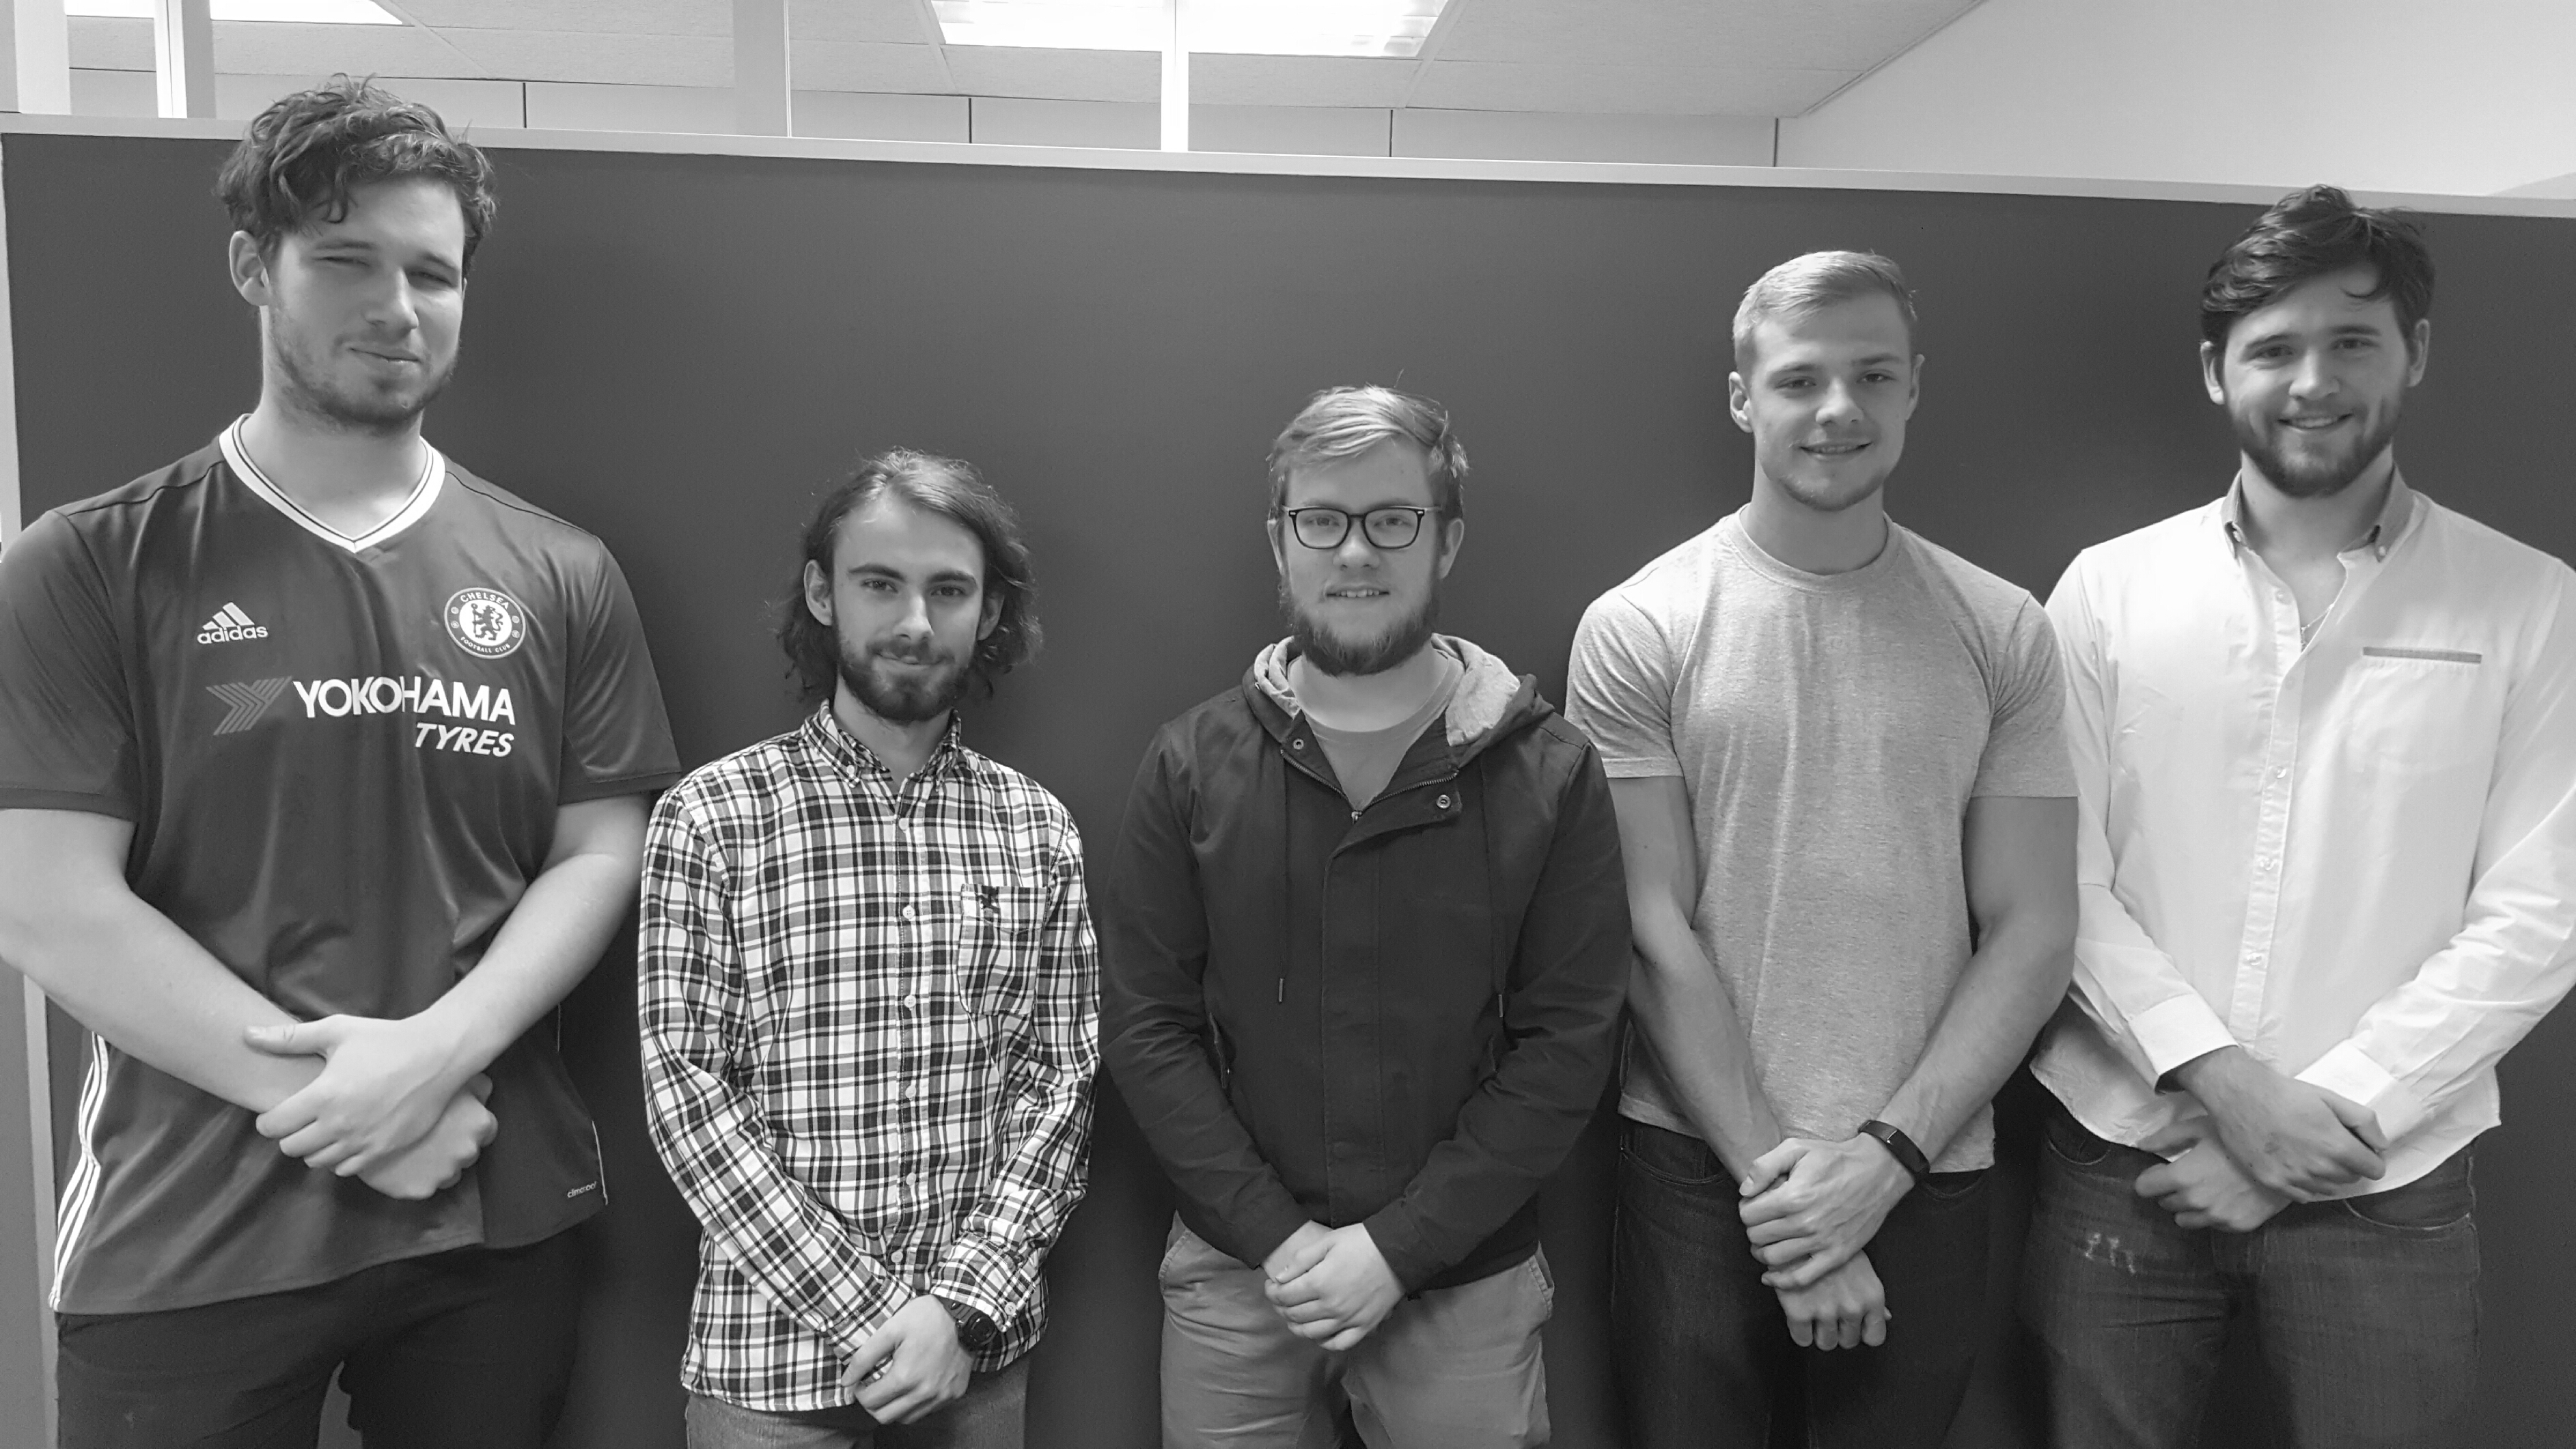
\includegraphics[width=\linewidth]{teamphoto.jpg}
	\end{figure}

	\begin{figure}[H]
		
\includegraphics[width=\linewidth]{teamtitle.jpg}
	\end{figure}

	\begin{figure}[H]
		
\includegraphics[width=\linewidth]{documenttitle.jpg}
	\end{figure}

	\begin{figure}[H]
		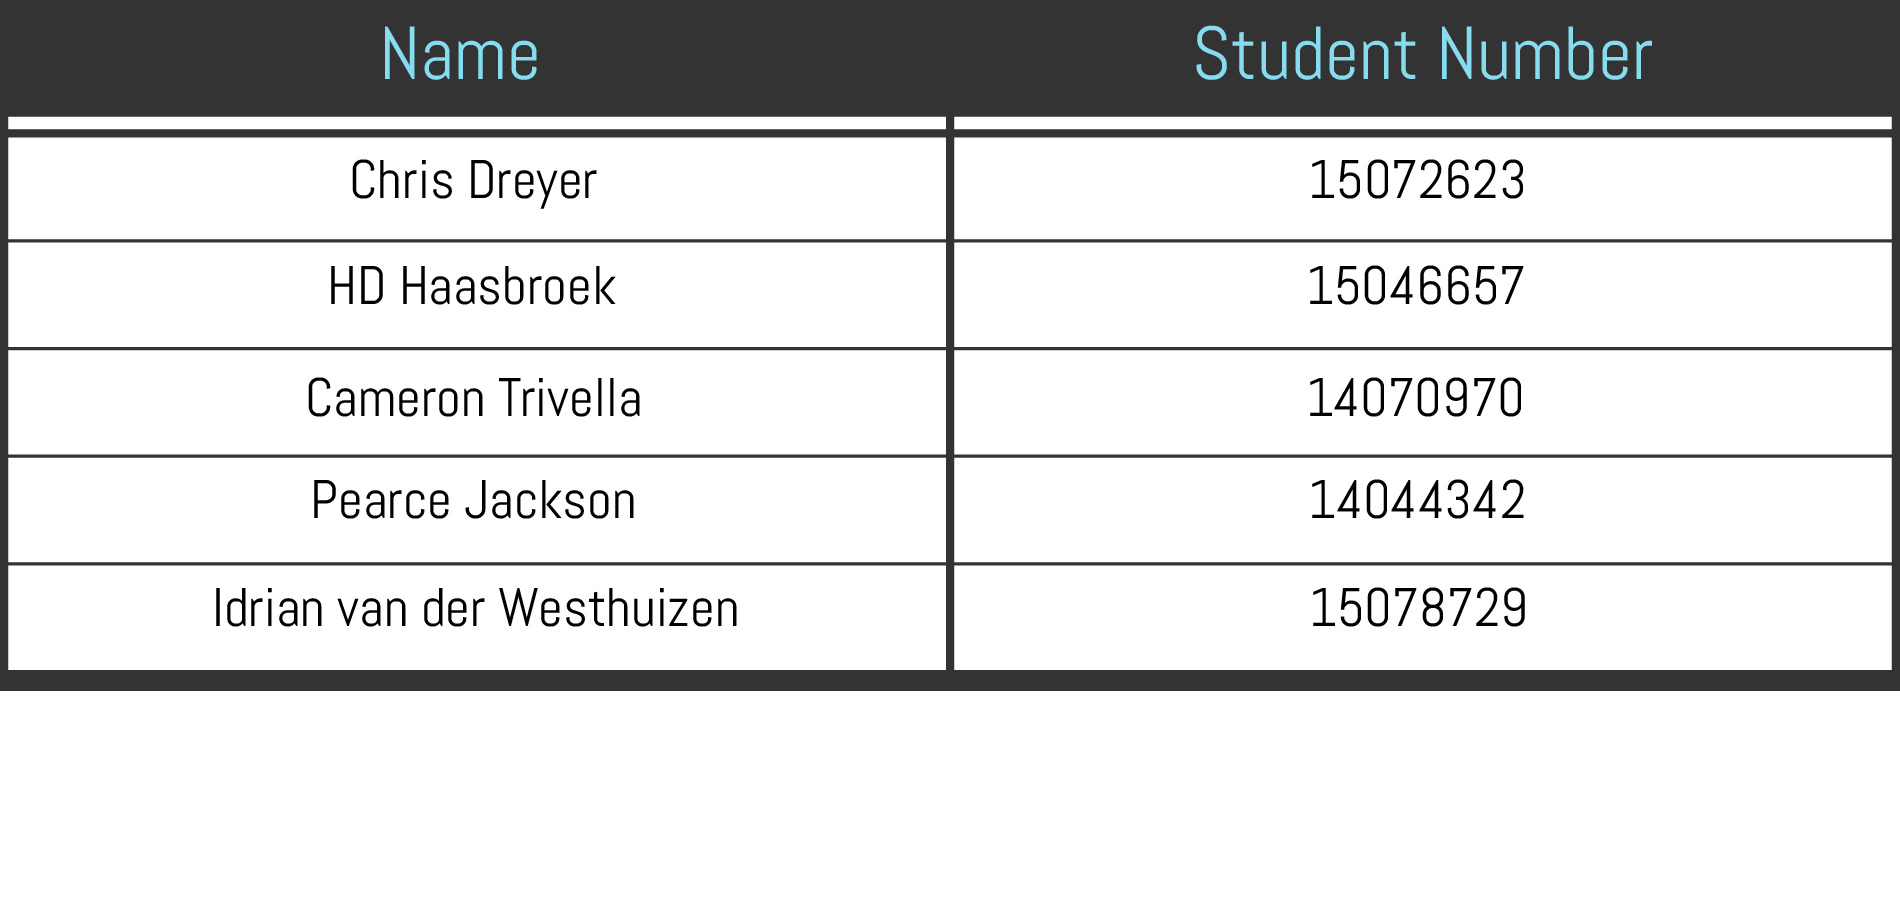
\includegraphics[width=\linewidth]{teamtable.jpg}
	\end{figure}
	
	\pagenumbering{gobble}
	\newpage
	\tableofcontents
	
	\pagenumbering{arabic}
	\newpage

	\section{Introduction}
	
		\subsection{Purpose}
		
		This SRS document aims to stipulate the requirements of the voxc.js library to aid in the development process and to ensure that a functional and usable product is delivered.
		
		\subsection{Product Scope}
		
		Voxc.js is meant to be an easy to use and easy to maintain JavaScript library, similar to how three.js is a library for WebGL. The purpose of the project is to provide users a way to import Voxel models into a webpage that would be using the Voxc.js library and ultimately texturing these Voxel models according to a rules file with a specified structure. The user will then be able to export the textured and rendered object.
		
		\subsection{References}
		
		\color{blue}
		\url{http://www.oskarstalberg.com/game/house/Index.html}
		\newline
		\\\url{https://voxel.codeplex.com/}
		\newline
		\\\url{https://pages.github.com/}
		\newline
		\\\url{http://threejs.org/}
		\newline
		\\\url{http://coffeescript.org/}
		\newline
		\\\url{http://es6-features.org/#Constants}
		\newline
		\\\url{http://www.typescriptlang.org/}
		\newline
		\\\url{http://www.codebelt.com/typescript/typescript-es6-modules-boilerplate/}
		\newline
		\\\url{http://giacomotag.io/typescript-webpack/}
		\color{black}
		
	\pagebreak
	
	\section{External Interface Requirements}
	
		\subsection{User Interfaces}
		The users will be interfacing with the Voxel system through online websites.*They will mainly be using a laptop or
		computer to interface with the system.* However the system itself will provide different interfaces for the user to make
		use of.
		
		This system does not require user profiles as their objects are only manipulate throught the system and not stored. This 
		implies that the user will only be led to one screen. On this screen they will be able to manipulate their objects.
		
		All users will share the same priority as there is not a distinction between user types. All users will have access to 
		all functions provided by the system.
		
		\subsection{Software Interfaces}
		The system will incorporate several different languages in order to function. For the rules file JSON objects will be 
		used so that the users can interface with the file. MagicVoxel will be used for the manipulation and movement of the 
		voxel objexts. The system will run off all major internet browsers that support WebGL.
		
		\subsection{Communications Interfaces}
		The system will have to handle frequent user uploads of their Voxel objects in order to manipulate them. *This
		communication can be done through any persistent internet connection*. Once the system has received communication from 
		the user it should access the rules file so as to be ready for the user interaction. This system should also allow 
		multiple users onto the system simultaneously. *This is to say that the system's performance should not be proportional 
		to the number of active users.*
		
	\pagebreak
	
	\section{System Features}
	
		\subsection{System Feature 1}
		
			 \subsubsection{Description and Priority}
			 
			 \subsubsection{Stimulus/Response Sequences}
			 
			 \subsubsection{Functional Requirements}
			 
	\pagebreak
	
	\section{Other Nonfunctional Requirements}
	
		\subsection{Performance Requirements}
		\subsubsection {Time to respond to an uploaded file}
		A user is required to upload a voxel object to the system and then will be allowed to mainpulate a rules file such that 
		their rules are now applied to the object. The system must not delay once a file is uploaded, this means a delay of no 
		more than *2 seconds* to respond to the upload should be allowed.
		
		\subsubsection{Respond to user interaction}
		Once the user has uploaded their object they may begin editing the object. The system should respond to the user 
		interaction in real time.
		
		\subsubsection{Reliability}
		The system should never cease working completely unless the error is caused
		by external systems outside our control (operating system, web APIs, etc).
		Ideally an entire system uptime (per month) of 99.9% must be reached.
		
		\subsubsection{Maintainability}
		The system’s code must be well documented, both by means of in-code comments and external documentation, to aid in 
		maintaining the system.
		
		\subsubsection{Portability}
		This system should be accessible across all major internet browsers that support WebGL. These include Chrome, Firefox 			etc.
		
		\subsubsection{Scalibilty}
		*It must be possible to scale the system backend in the event of an increase of users. Scaling must be possible both 
		horizontally or vertically.*
		
		\subsubsection{Usability}
		The Voxel system should be easy to operate and understand. The core functions of the system shouldn't take the user more 
		than a minute to access and understand.
		
		\subsection{Security Requirements}
		This system should be an open source project and so the code should be freely available to anyone seeking the code.
		However the actual system should be protected and the only editing that a user can do is uploading of objects and 
		editing of the rules file.
		
		\subsection{Quality Requirements}
		********************************************************
		
	\pagebreak
	
\end{document}
